\documentclass[UTF8, letter]{article}

\usepackage[margin=1in]{geometry}
\usepackage{graphicx}
\usepackage{lipsum}
\usepackage[framemethod=tikz]{mdframed}
\usepackage{minted}
\usepackage{setspace}
\usepackage{xcolor}
\usepackage{subcaption}
\usemintedstyle{xcode}

\definecolor{codebg}{RGB}{192,199,209}

\mdfdefinestyle{codeframe}{
	backgroundcolor=codebg,
	linewidth=0,
	skipbelow=-10,
}
\newmdenv[style=codeframe,%
	settings={\singlespacing}]{codeblock}

\title{Programming Assignment 2 \\
\large INFO-5502 (Section 002): \\
Analytic Tools, Techniques and Methods }
\author{Ramandeep Harjai}



\begin{document}
\maketitle

\doublespacing
\setlength{\parskip}{\baselineskip}
\setlength{\parindent}{4em}

\begin{codeblock}
\begin{minted}{python}
!pip install datascience

from datascience import Table
import matplotlib.pyplot as plt
import math
\end{minted}
\end{codeblock}

\vspace{5mm}
\begin{codeblock}
\begin{minted}{python}
# load HIV data 
data_url = 'https://raw.githubusercontent.com/rdharjai/info5502/main/hw2/hiv.csv'
hiv_full_tbl = Table.read_table(data_url)

print('\nTable loaded with: {} rows\n'.format(hiv_full_tbl.num_rows))
hiv_full_tbl
\end{minted}
\end{codeblock}

\vspace{5mm}
\begin{figure}[h!]
	\centering
	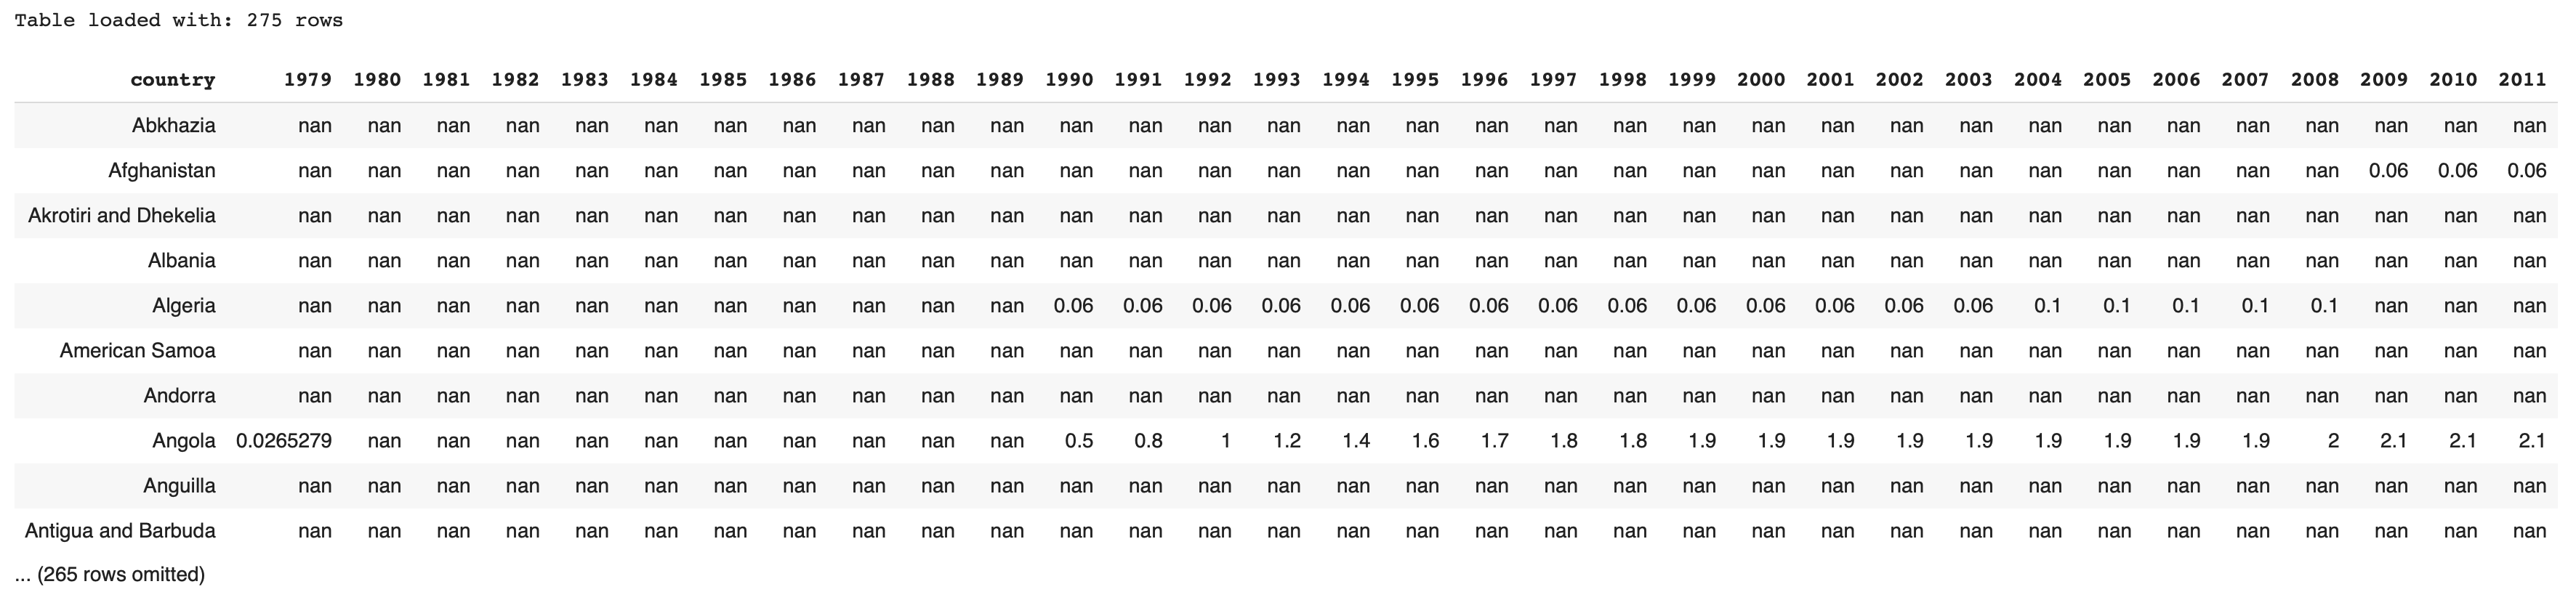
\includegraphics[width=\linewidth]{output_1.png}
	\caption{HIV data - loaded raw data}
	\label{fig:boat1}
\end{figure}


\pagebreak
\begin{codeblock}
\begin{minted}{python}
# convert empty or NAN values to 0
cols = list(hiv_full_tbl.labels)
cols.remove('country')
for _ in range(len(cols)):
  hiv_full_tbl = hiv_full_tbl.with_column(cols[_], 
            hiv_full_tbl.apply(lambda x: 0 if (math.isnan(x)) else x, cols[_]))

print('\nEmpty cells (NAN values) converted to 0 value.')
print('\nTable loaded with: {} rows\n'.format(hiv_full_tbl.num_rows))
hiv_full_tbl
\end{minted}
\end{codeblock}

\begin{figure}[h!]
	\centering
	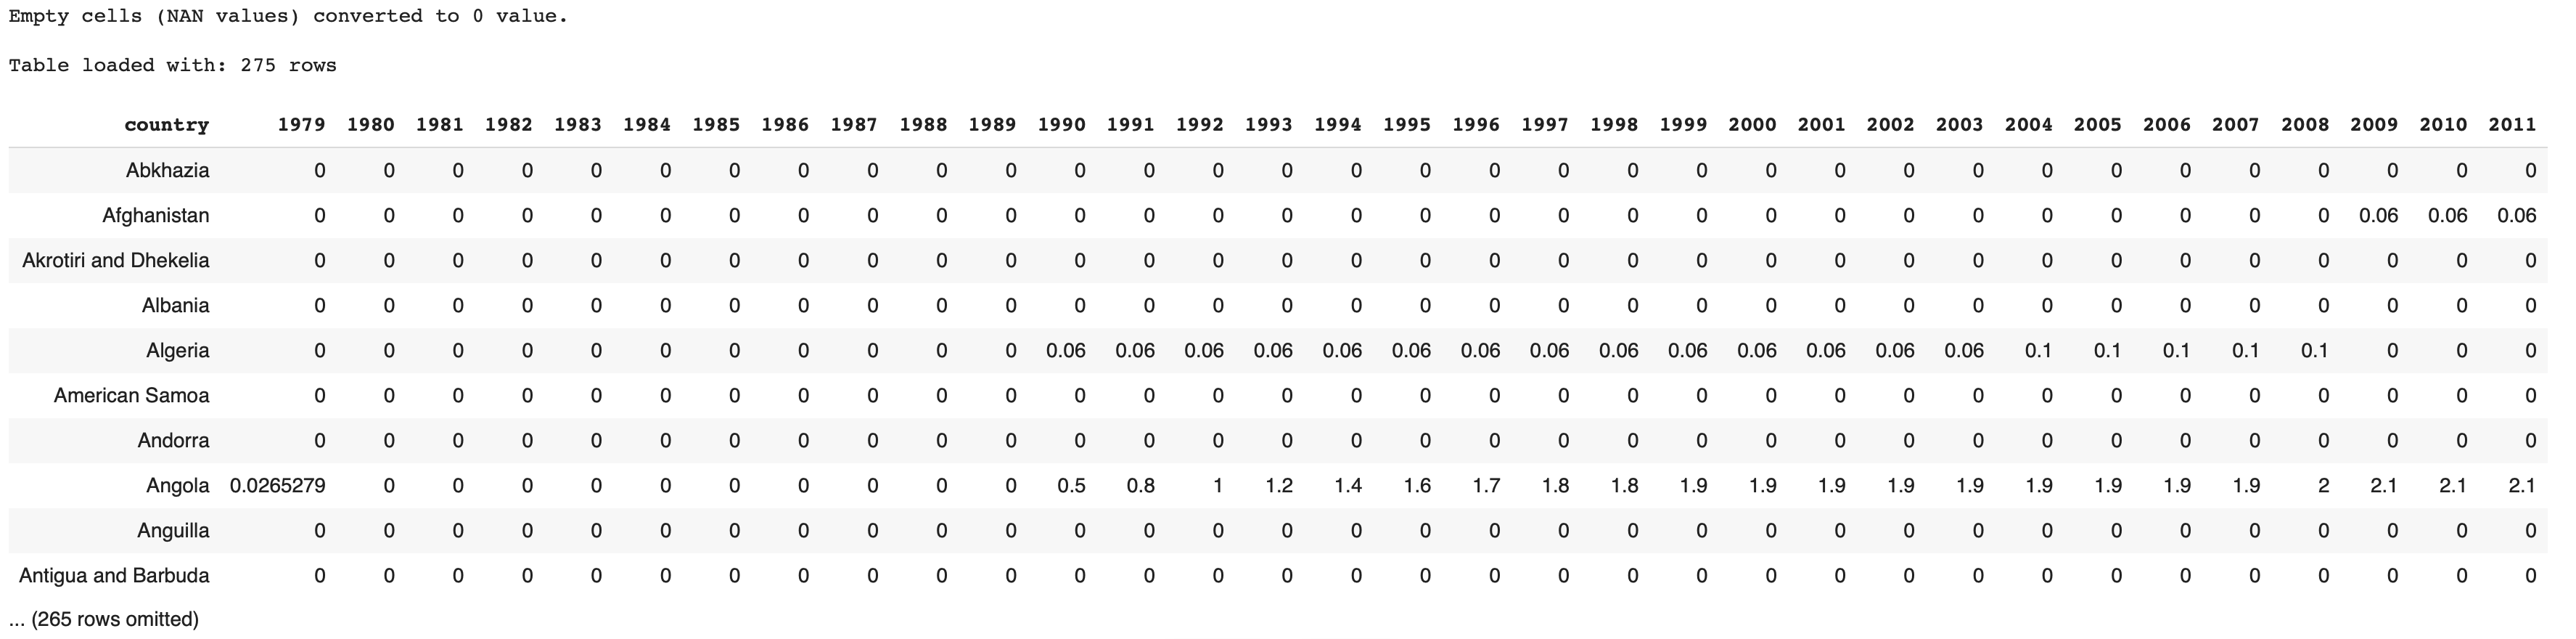
\includegraphics[width=\linewidth]{output_2.png}
	\caption{HIV data - Converted NAN values to 0}
	\label{fig:boat1}
\end{figure}

\vspace{5mm}
\begin{codeblock}
\begin{minted}{python}
# remove rows with no data
# i.e. rows with all 0 values
# hiv_tbl2 = hiv_tbl.copy(shallow=False)
empty_row = (0.0, 0.0, 0.0, 0.0, 0.0, 0.0, 0.0, 0.0, 0.0, 0.0, 0.0, 
             0.0, 0.0, 0.0, 0.0, 0.0, 0.0, 0.0, 0.0, 0.0, 0.0, 0.0, 
             0.0, 0.0, 0.0, 0.0, 0.0, 0.0, 0.0, 0.0, 0.0, 0.0)
empty_row_idxs = []
row_idx = 0
for row in hiv_full_tbl.rows:
  if tuple(row[1:-1]) == empty_row:
    empty_row_idxs.append(row_idx)
  row_idx += 1

print('\n{} null rows found & removed.'.format(len(empty_row_idxs)))
hiv_tbl = hiv_full_tbl.exclude(empty_row_idxs)

print('\nTable loaded with: {} rows\n'.format(hiv_tbl.num_rows))
hiv_tbl\end{minted}
\end{codeblock}

\begin{figure}[h!]
	\centering
	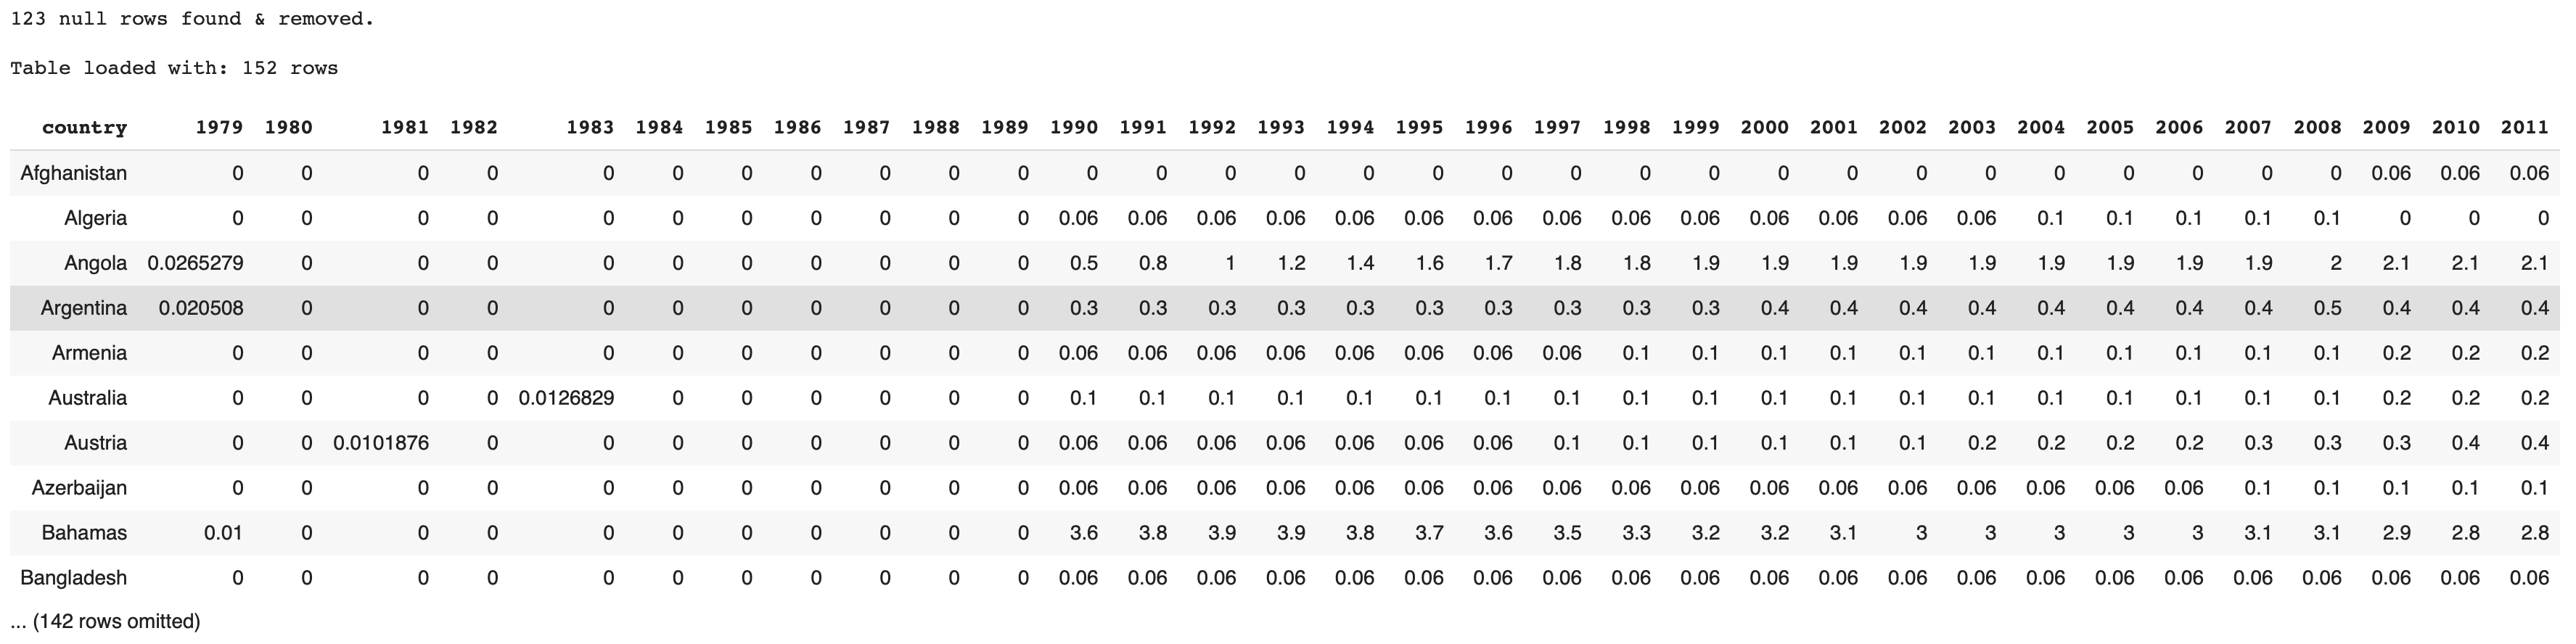
\includegraphics[width=\linewidth]{output_3.png}
	\caption{HIV data - removed null rows}
	\label{fig:boat1}
\end{figure}



\pagebreak
\paragraph{Task \#1}
Add one column as “continent” in the dataset and label each country/region in the dataset to an appropriate continent such as “Europe”, “Asia”, “Africa”, “North America”, “South America”, “Australia”, or “Antarctica”. Explain how do validated the correctness of your labelling. Output the updated dataset as a new CSV file. (1 point). (Note: You must write a Python program to complete the labelling, manually labelling will not get any credit).

\begin{codeblock}
\begin{minted}{python}
# load country-continent data
country_data_url = 'https://raw.githubusercontent.com/rdharjai/info5502/' \
'main/hw2/country.csv'
country_tbl = Table.read_table(country_data_url)

# join HIV table with Country table
hiv_tbl = hiv_tbl.join('country', country_tbl, 'country')

# move the country & continent column 
# as the first 2 columns in table
hiv_tbl.move_to_start('continent')
hiv_tbl.move_to_start('country')

# print table to validate country-continent names
print(hiv_tbl)
print("\nRows without continent label: ", hiv_tbl.where('continent','').num_rows)

# export data-table as a CSV file 
hiv_tbl.to_csv('hiv_tbl.csv')

# smoke test to validate correctness of the 
# continent labelling
assert(hiv_tbl.where('country','India').column('continent')=='Asia')
assert(hiv_tbl.where('country','Japan').column('continent')=='Asia')
assert(hiv_tbl.where('country','Canada').column('continent')=='North America')
assert(hiv_tbl.where('country','United States').column('continent')=='North America')
assert(hiv_tbl.where('country','Argentina').column('continent')=='South America')
assert(hiv_tbl.where('country','Brazil').column('continent')=='South America')
assert(hiv_tbl.where('country','Australia').column('continent')=='Oceania')
assert(hiv_tbl.where('country','New Zealand').column('continent')=='Oceania')
print("Smoke test for conuntry-continent labelling has passed successfully.")
\end{minted}
\end{codeblock}

\begin{figure}[h!]
	\centering
	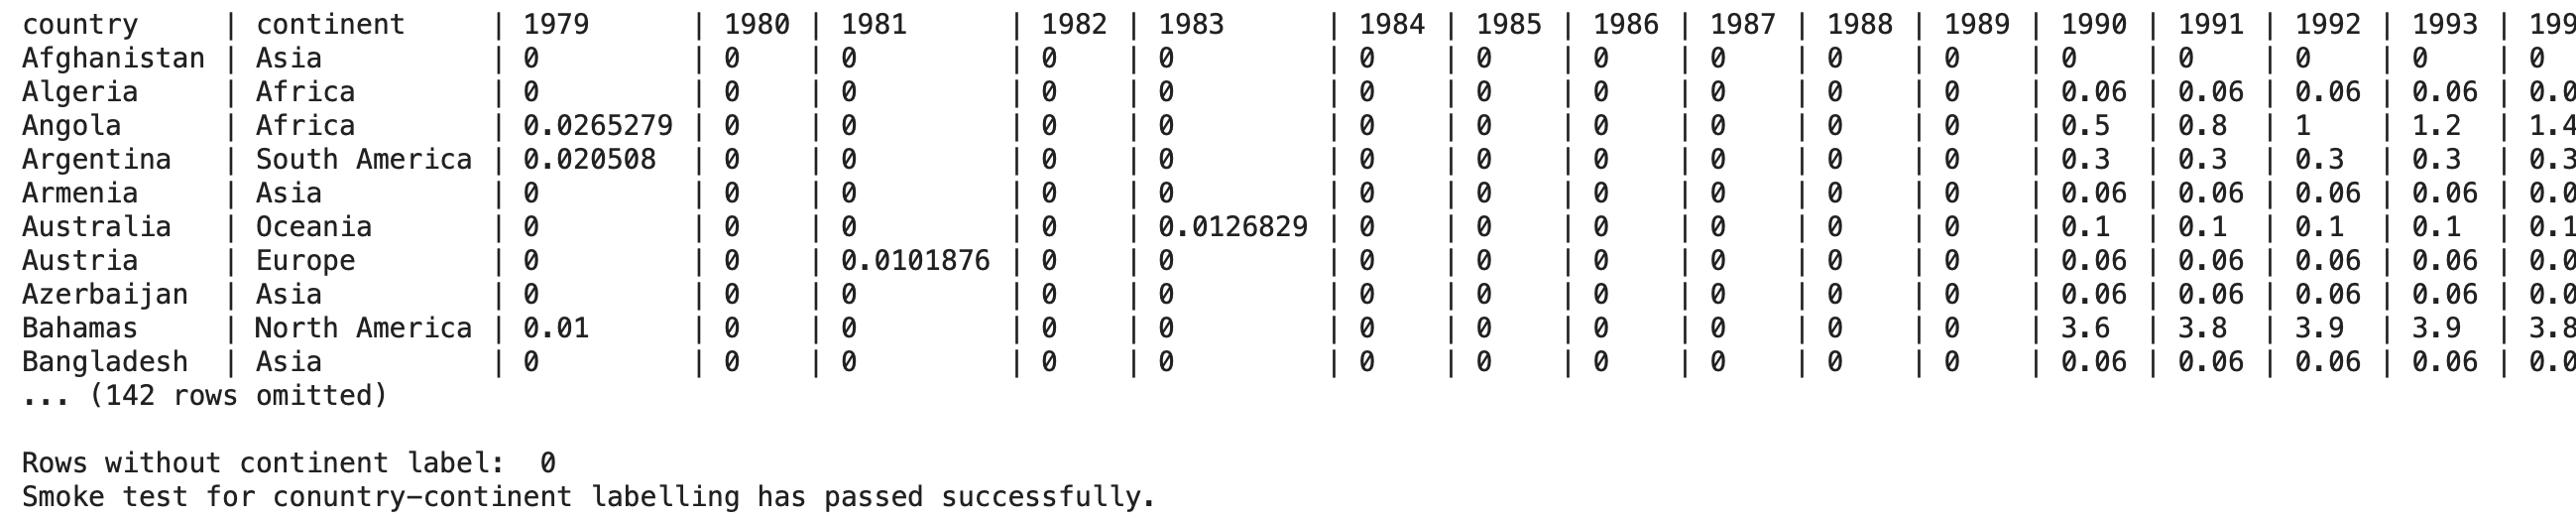
\includegraphics[width=\linewidth]{output_4.png}
	\caption{HIV data - Joined country-continent data}
	\label{fig:boat1}
\end{figure}

\pagebreak
\paragraph{Task \#2}
Write a Python program to find the country/region in each continent that has the highest average HIV estimated prevalence of people ages from 15 to 49 of from year 2000 to 2011. Find the country/region in each continent that has the lowest average HIV estimated prevalence of people ages from 15 to 49 of from year 2000 to 2011. Create a bar chart to show the highest average HIV estimated prevalence of people ages from 15 to 49 of from year 2000 to 2011 in each continent (1 point). Create a bar chart to show the lowest average HIV estimated prevalence of people ages from 15 to 49 of from year 2000 to 2011 in each continent (1 point). Create an overlaid bar chart to show the highest and lowest average HIV estimated prevalence of people ages from 15 to 49 of from year 2000 to 2011 in each continent (1 point). Select a country/region that is different from the average highest or lowest HIV estimated prevalence of people ages from 15 to 49 from year 2000 to 2011 from each continent, then create an overlaid line chart for the selected country/region, the average highest and lowest HIV estimated prevalence of people ages from 15 to 49 from year 2000 to 2011 for each continent (1 point).

\begin{codeblock}
\begin{minted}{python}
# add a new column: 2000_2011_avg
# it is the average of values of all columns 
# between 2000 (index: 23) and 2011 (index: 34)

avg_lst = []
for row in hiv_tbl.rows:
  avg_lst.append(round(sum(list(row)[23:35]) / len(list(row)[23:35]),3))

try:
  hiv_tbl.drop('2000_2011_avg')
finally:
  hiv_tbl = hiv_tbl.with_column('2000_2011_avg', avg_lst)

hiv_tbl
\end{minted}
\end{codeblock}

\begin{figure}[h!]
	\centering
	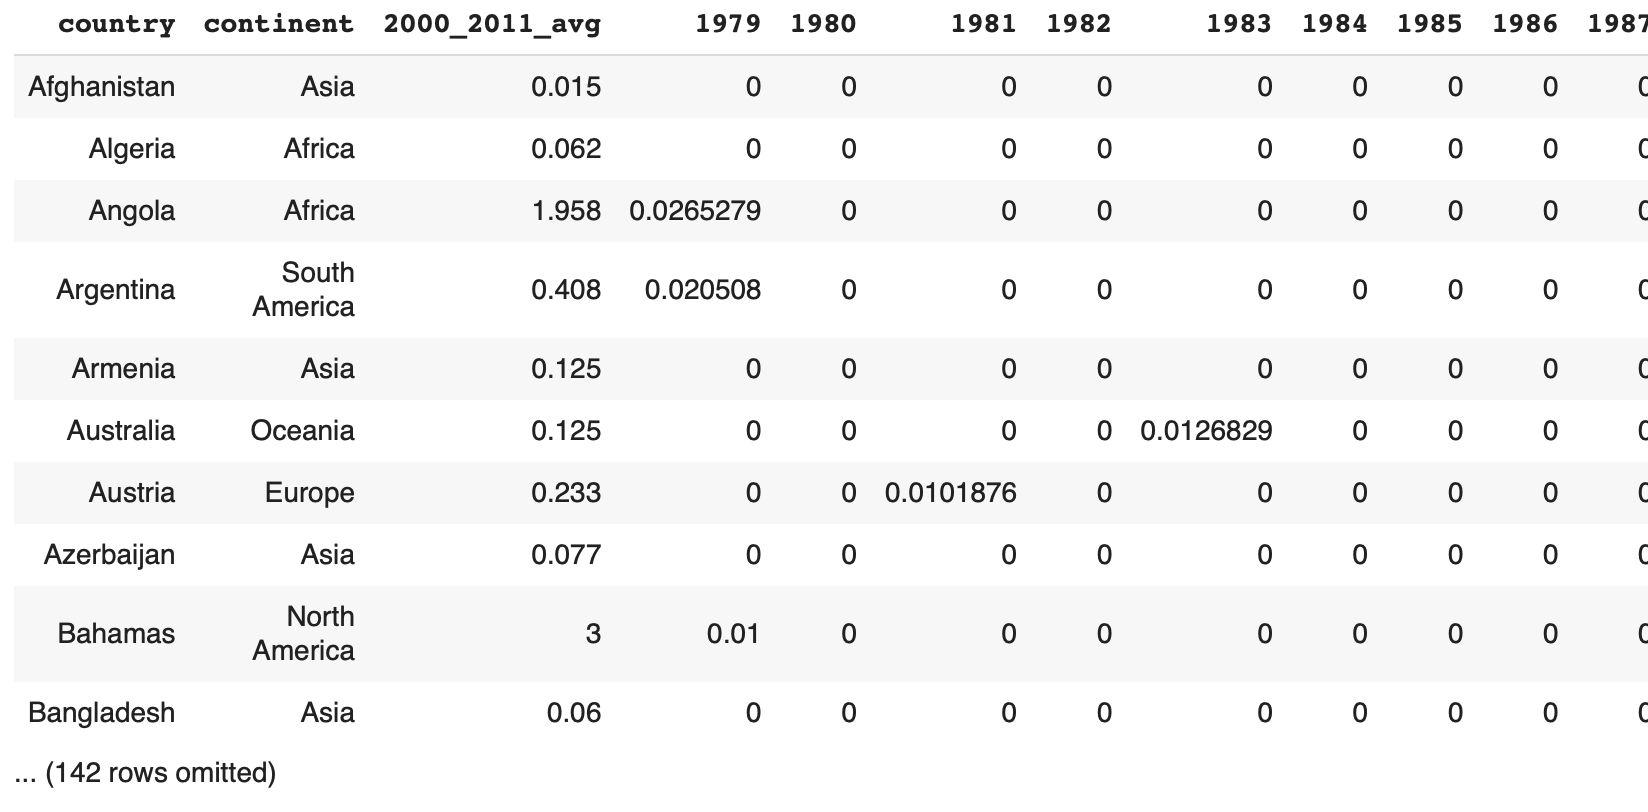
\includegraphics[width=0.8\linewidth]{output_5.png}
	\caption{HIV data - Added column for avg. of 2000-2011}
	\label{fig:boat1}
\end{figure}

\pagebreak
\begin{codeblock}
\begin{minted}{python}
lst_2000_2011_avg_high = []
for row in hiv_tbl.group('continent', max).select(0,35).sort('2000_2011_avg max', descending = True).rows:
  lst_2000_2011_avg_high.append(tuple(hiv_tbl
                                      .where('continent',row[0])
                                      .where('2000_2011_avg',row[1])
                                      .select(1,0,35)
                                      .row(0)))

print('\nCountry/region in each continent that has the highest average HIV ', 
      '\nestimated prevalence of people ages from 15 to 49 of ',
      '\nfrom year 2000 to 2011\n')

print('{:<20} {:<20} {:>5}'.format('Continent', 'Country', 'HIV Avg.'))
print('{:<20} {:<20} {:>5}'.format('---------', '-------', '--------'))
for item in lst_2000_2011_avg_high:
  print('{:<20} {:<20} {:>5.2f}'.format(item[0],item[1],item[2]))
\end{minted}
\end{codeblock}

\begin{figure}[h!]
	\centering
	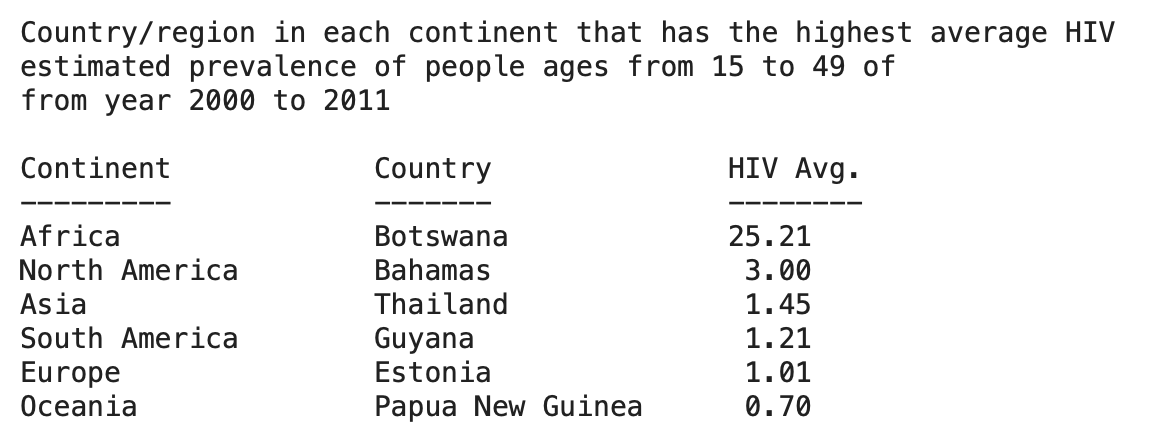
\includegraphics[width=\linewidth]{output_6.png}
	\caption{HIV data - highest average data for 2000-2011 by continents}
	\label{fig:boat1}
\end{figure}

\pagebreak
\begin{codeblock}
\begin{minted}{python}
lst_2000_2011_avg_low = []
for row in hiv_tbl.group('continent', min).select(0,35).sort('2000_2011_avg min').rows:
  lst_2000_2011_avg_low.append(tuple(hiv_tbl
                                      .where('continent',row[0])
                                      .where('2000_2011_avg',row[1])
                                      .select(1,0,35)
                                      .row(0)))

print('\nCountry/region in each continent that has the lowest average HIV ', 
      '\nestimated prevalence of people ages from 15 to 49 of ',
      '\nfrom year 2000 to 2011\n')

print('{:<20} {:<20} {:>5}'.format('Continent', 'Country', 'HIV Avg.'))
print('{:<20} {:<20} {:>5}'.format('---------', '-------', '--------'))
for item in lst_2000_2011_avg_low:
  print('{:<20} {:<20} {:>5.2f}'.format(item[0],item[1],item[2]))\end{minted}
\end{codeblock}

\begin{figure}[h!]
	\centering
	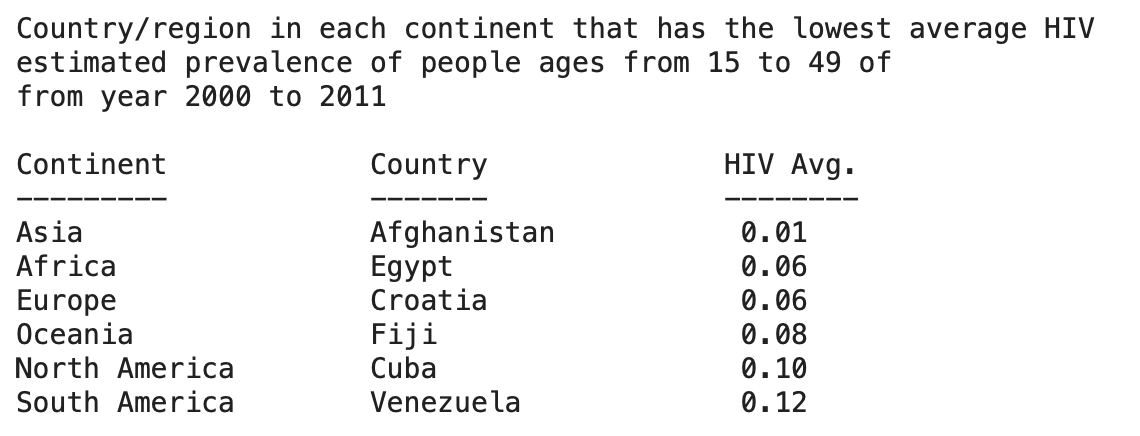
\includegraphics[width=\linewidth]{output_7.png}
	\caption{HIV data - lowest average data for 2000-2011 by continents}
	\label{fig:boat1}
\end{figure}

\pagebreak
\begin{codeblock}
\begin{minted}{python}
x_val = [x[0] for x in lst_2000_2011_avg_high]
y_high_val = [x[2] for x in lst_2000_2011_avg_high]

fig, (ax1) = plt.subplots(1,1,constrained_layout=True)
fig.set_size_inches(8, 6)
fig.set_dpi(100)
fig.suptitle('highest average HIV estimated prevalence of people ages from \
15 to 49 \n from year 2000 to 2011 in each continent \n (using log scale)')

# Bar Plot 
ax1.set_yscale('log')
ax1.set(xlabel='Continents', 
        ylabel='Average HIV estimated prevalence \n (in log scale)')
ax1.bar(x_val, 
        y_high_val,
        label="Highest avg. HIV estimated prevalence")
ax1.legend()
\end{minted}
\end{codeblock}

\begin{figure}[h!]
	\centering
	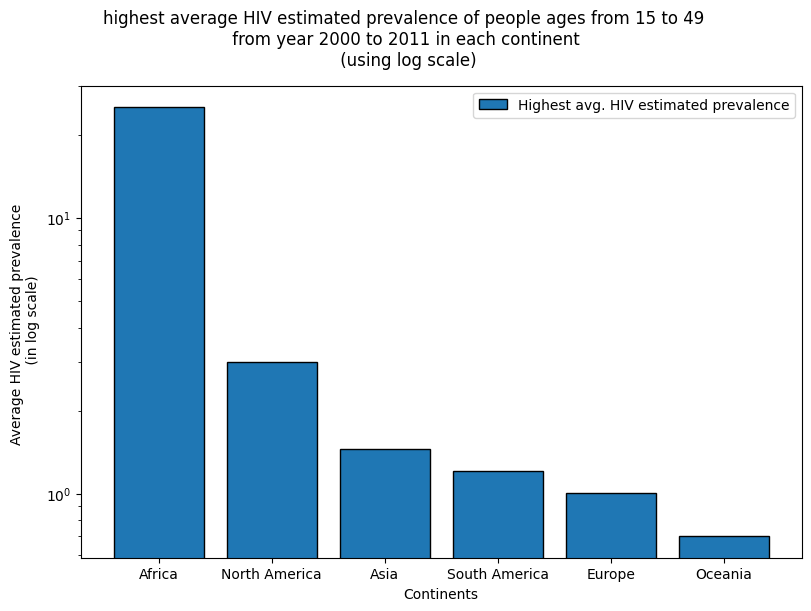
\includegraphics[width=0.9\linewidth]{output_8.png}
	\caption{HIV data - bar chart for highest average data for 2000-2011 by continents}
	\label{fig:boat1}
\end{figure}

\pagebreak
\begin{codeblock}
\begin{minted}{python}
x_val = [x[0] for x in lst_2000_2011_avg_low]
y_low_val = [x[2] for x in lst_2000_2011_avg_low]

fig, (ax1) = plt.subplots(1,1,constrained_layout=True)
fig.set_size_inches(8, 6)
fig.set_dpi(100)
fig.suptitle('lowest average HIV estimated prevalence of people ages from \
15 to 49 \n from year 2000 to 2011 in each continent \n (using log scale)')

# Bar Plot 
ax1.set_yscale('log')
ax1.set(xlabel='Continents', 
        ylabel='Average HIV estimated prevalence \n (in log scale)')
ax1.bar(x_val, 
        y_low_val,
        label="Lowest avg. HIV estimated prevalence")

ax1.legend()
\end{minted}
\end{codeblock}

\begin{figure}[h!]
	\centering
	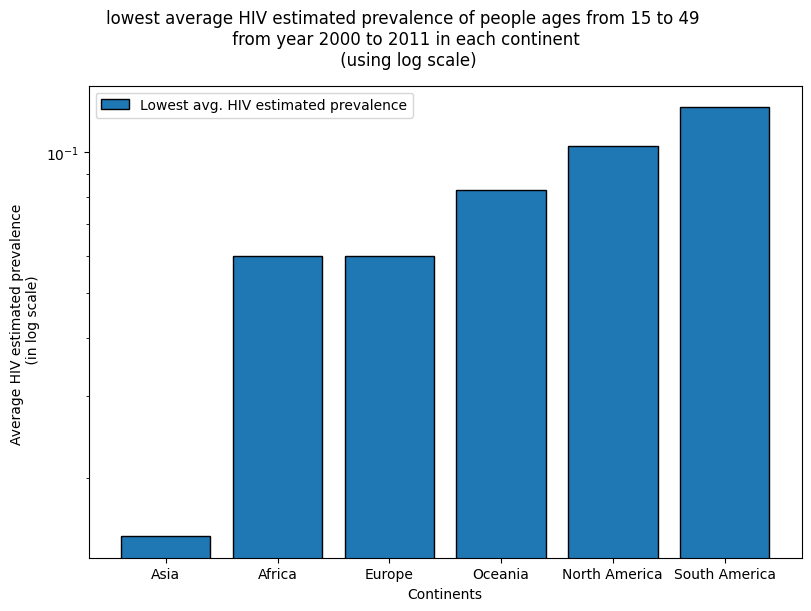
\includegraphics[width=0.9\linewidth]{output_9.png}
	\caption{HIV data - bar chart for lowest average data for 2000-2011 by continents}
	\label{fig:boat1}
\end{figure}

\pagebreak
\begin{codeblock}
\begin{minted}{python}
fig, (ax1) = plt.subplots(1,1,constrained_layout=True)
fig.set_size_inches(8, 6)
fig.set_dpi(100)
fig.suptitle('highest & lowest average HIV estimated prevalence of people ages from \
15 to 49 \n from year 2000 to 2011 in each continent \n (using log scale)')

# Bar Plot 
ax1.set_yscale('log')
ax1.set(xlabel='Continents', 
        ylabel='Average HIV estimated prevalence \n (in log scale)')

ax1.bar(x_val, 
        y_high_val, 
        width=0.9, 
        label="Highest avg. HIV estimated prevalence")

ax1.bar(x_val, 
        y_low_val, 
        width=0.7, 
        label="Lowesr avg. HIV estimated prevalence")

ax1.legend()
\end{minted}
\end{codeblock}

\begin{figure}[h!]
	\centering
	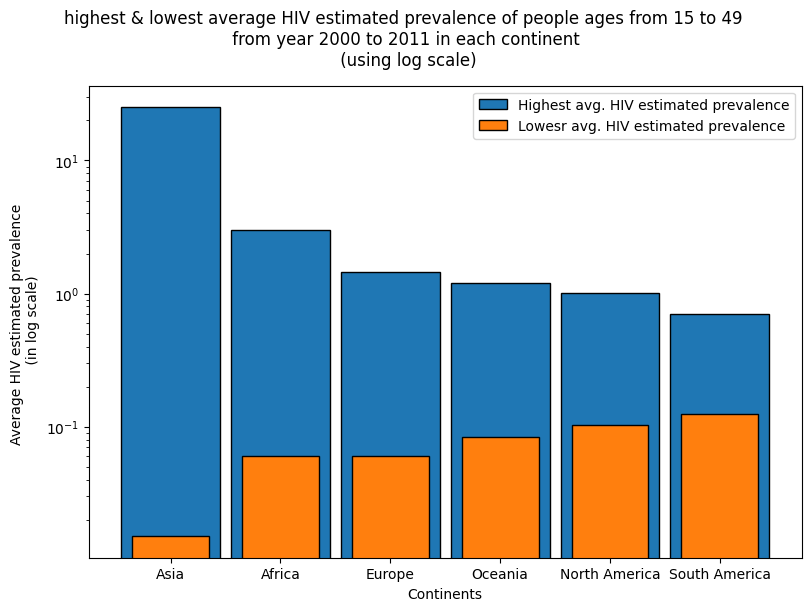
\includegraphics[width=0.9\linewidth]{output_10.png}
	\caption{HIV data - bar chart for highest \& lowest average data for 2000-2011 by continents}
	\label{fig:boat1}
\end{figure}

\pagebreak
\paragraph{Task \#3}
Write a Python program to calculate the average HIV estimated prevalence of people ages from 15 to 49 for each year in the dataset for each continent (you only need simply add the estimate prevalence number of all countries/regions and divided by the number of the countries/regions in the continent). Based on the calculation, create a line chart for each continent to show the changes of the average HIV estimated prevalence from 1979 to 2011 (1 point). Create an overlaid line chart for all continents to show their changes of the average HIV estimated prevalence from 1 1979 to 2011 (1 point).

\begin{codeblock}
\begin{minted}{python}
lst_continents = []
for row in hiv_tbl.group('continent').rows:
  lst_continents.append(tuple(row))

lst_year_avg = []
for continent in lst_continents:
  lst = []
  for col in range(2, hiv_tbl.num_columns-1):
    lst.append((hiv_tbl.labels[col], 
                round(hiv_tbl.where('continent',continent[0]).select(col)
                .mean()
                .row(0)[0],3)))
  lst_year_avg.append([continent[0],lst])


fig, axs = plt.subplots(len(lst_year_avg),1,constrained_layout=True)
fig.set_size_inches(8, 20)
fig.set_dpi(100)
fig.suptitle('Changes of the average HIV estimated prevalence \
\n from 1979 to 2011 for each continent')

idx = 0
for ax in axs:
  x_data = [x[0] for x in lst_year_avg[idx][1]]
  y_data = [x[1] for x in lst_year_avg[idx][1]]
  ax.set(xlabel='Year', 
        ylabel='Average HIV estimated prevalence \n (in log scale)')
  ax.set_xticklabels(x_data, rotation=90)
  ax.plot(x_data, y_data, label=lst_year_avg[idx][0])
  ax.legend()
  idx += 1
\end{minted}
\end{codeblock}

\begin{figure}
	\centering
	\begin{subfigure}[b]{1\textwidth}
		\centering
		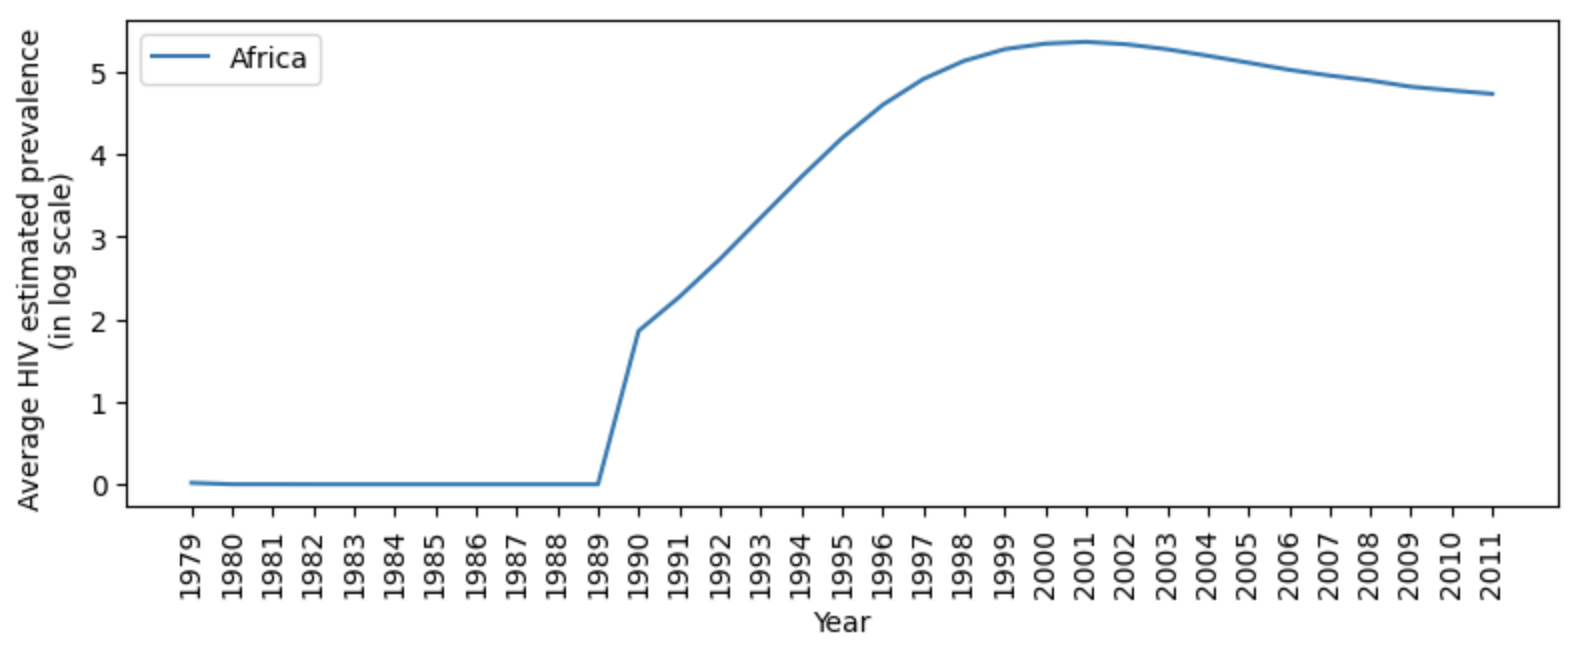
\includegraphics[width=\linewidth]{output_12.png}
		\caption{HIV data - Africa: Changes of the average HIV estimated prevalence from 1979 to 2011 for each continent}
		\label{fig:line1}		
	\end{subfigure}
	\begin{subfigure}[b]{1\textwidth}
		\centering
		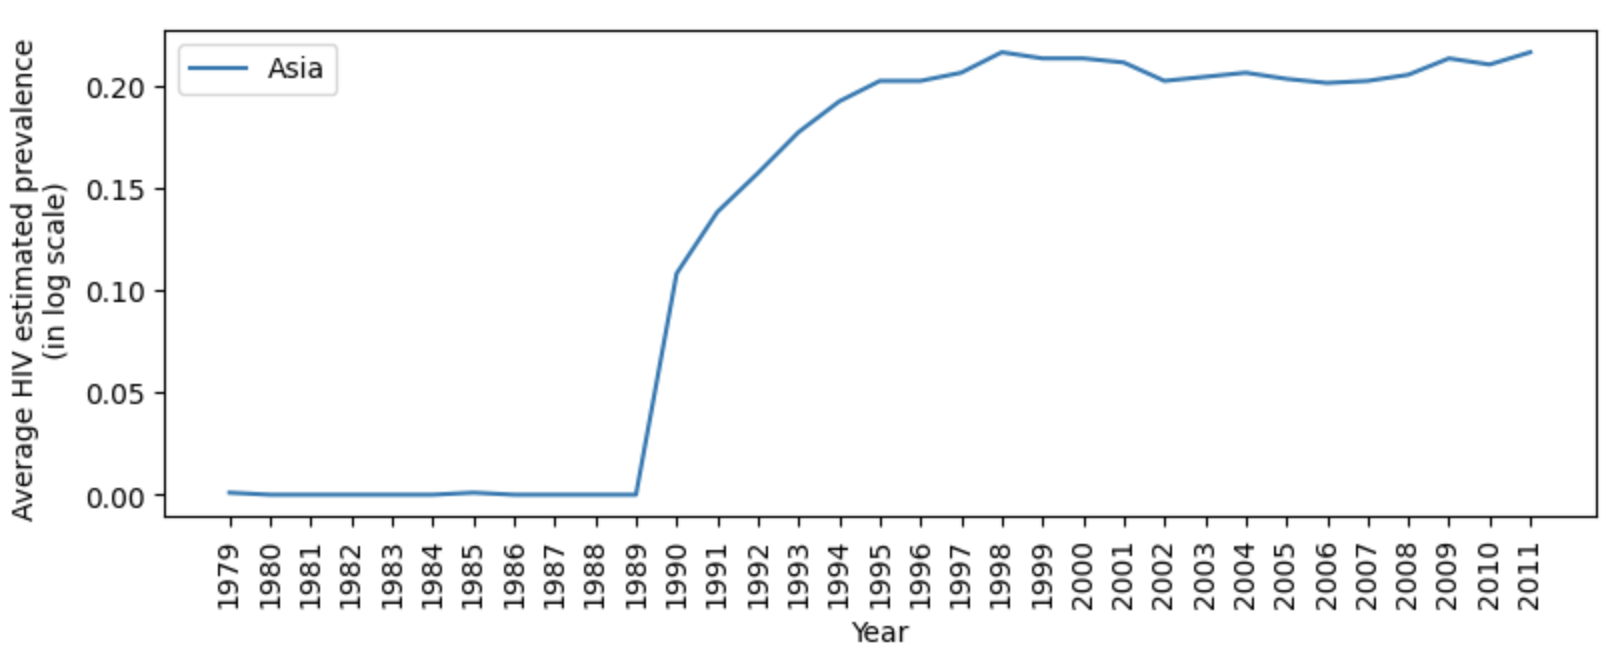
\includegraphics[width=\linewidth]{output_13.png}
		\caption{HIV data - Asia: Changes of the average HIV estimated prevalence from 1979 to 2011 for each continent}
		\label{fig:line1}		
	\end{subfigure}
	\begin{subfigure}[b]{1\textwidth}
		\centering
		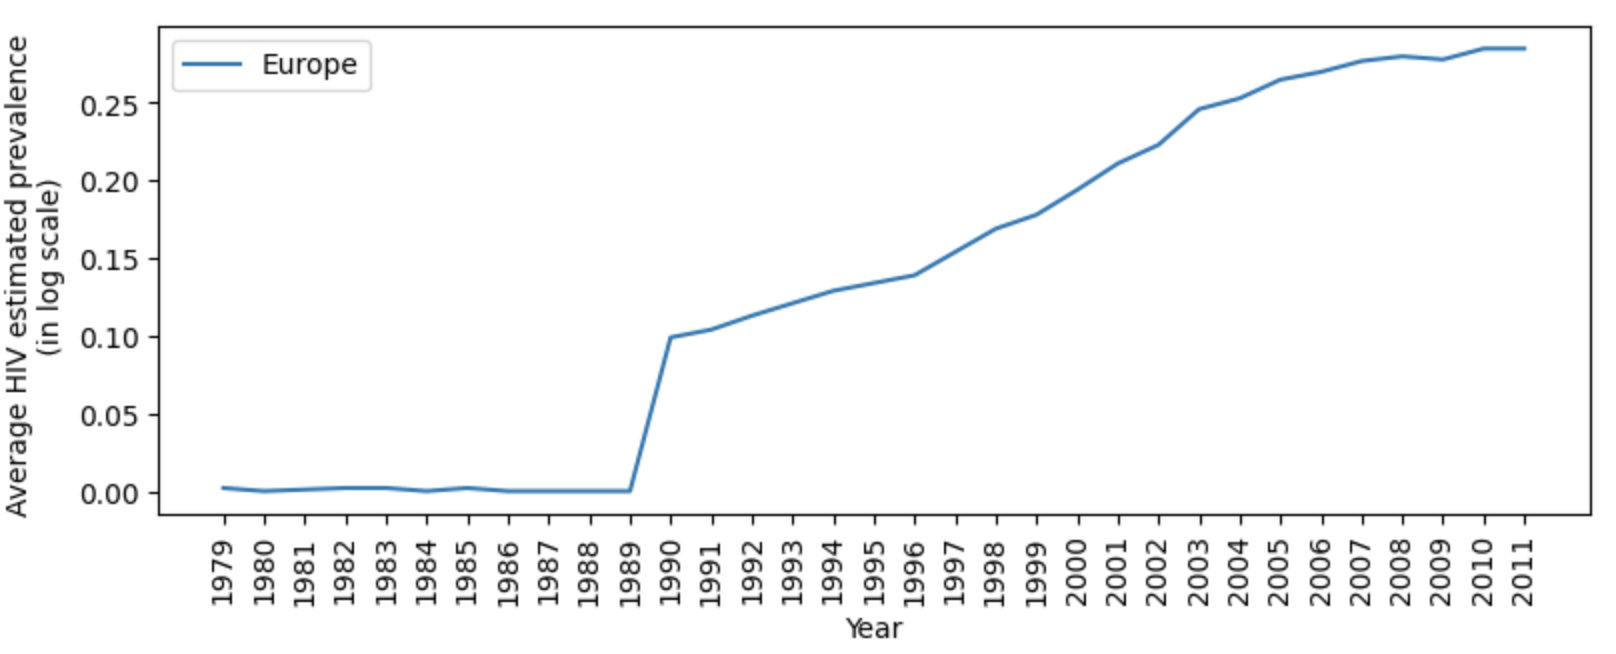
\includegraphics[width=\linewidth]{output_14.png}
		\caption{HIV data - Europe: Changes of the average HIV estimated prevalence from 1979 to 2011 for each continent}
		\label{fig:line1}		
	\end{subfigure}				
\end{figure}

\begin{figure}
	\centering
	\begin{subfigure}[b]{1\textwidth}
		\centering
		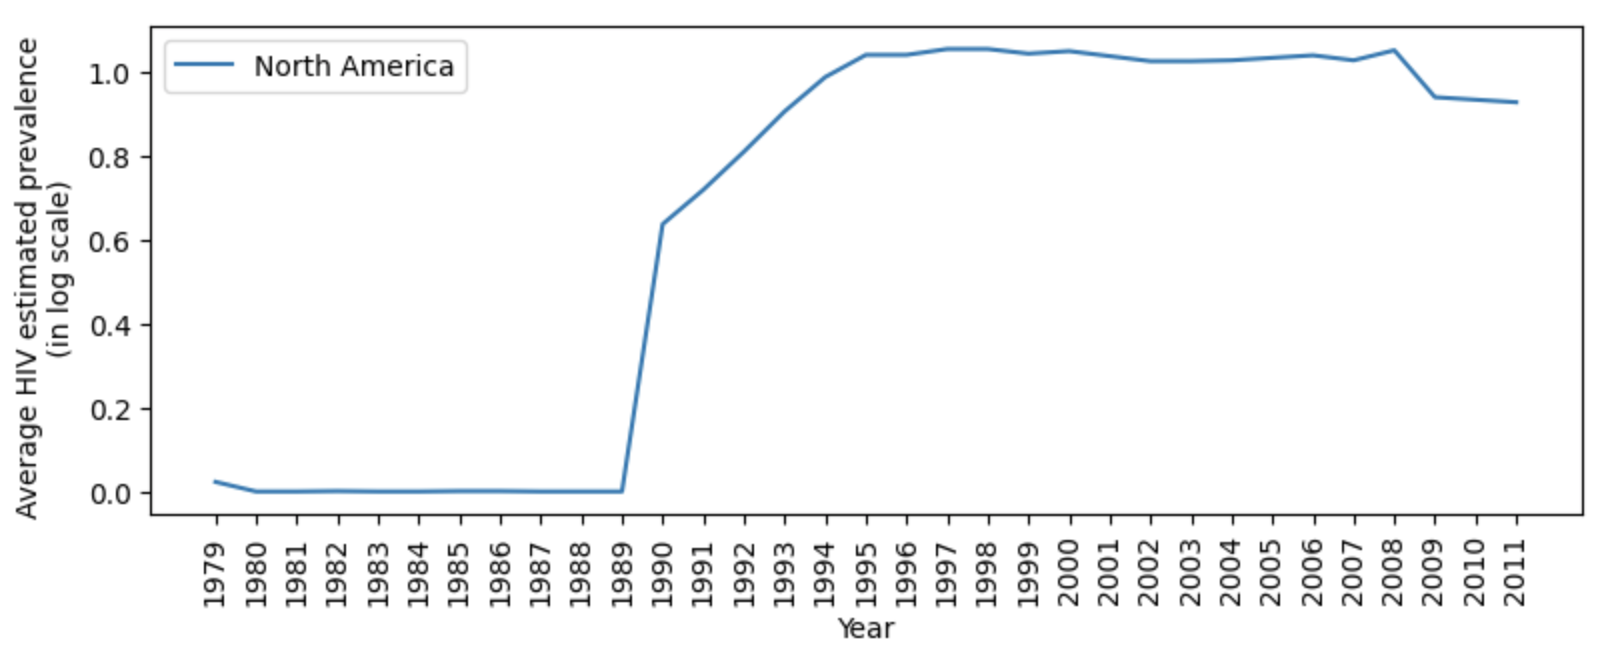
\includegraphics[width=\linewidth]{output_15.png}
		\caption{HIV data - North America: Changes of the average HIV estimated prevalence from 1979 to 2011 for each continent}
		\label{fig:line1}		
	\end{subfigure}
	\begin{subfigure}[b]{1\textwidth}
		\centering
		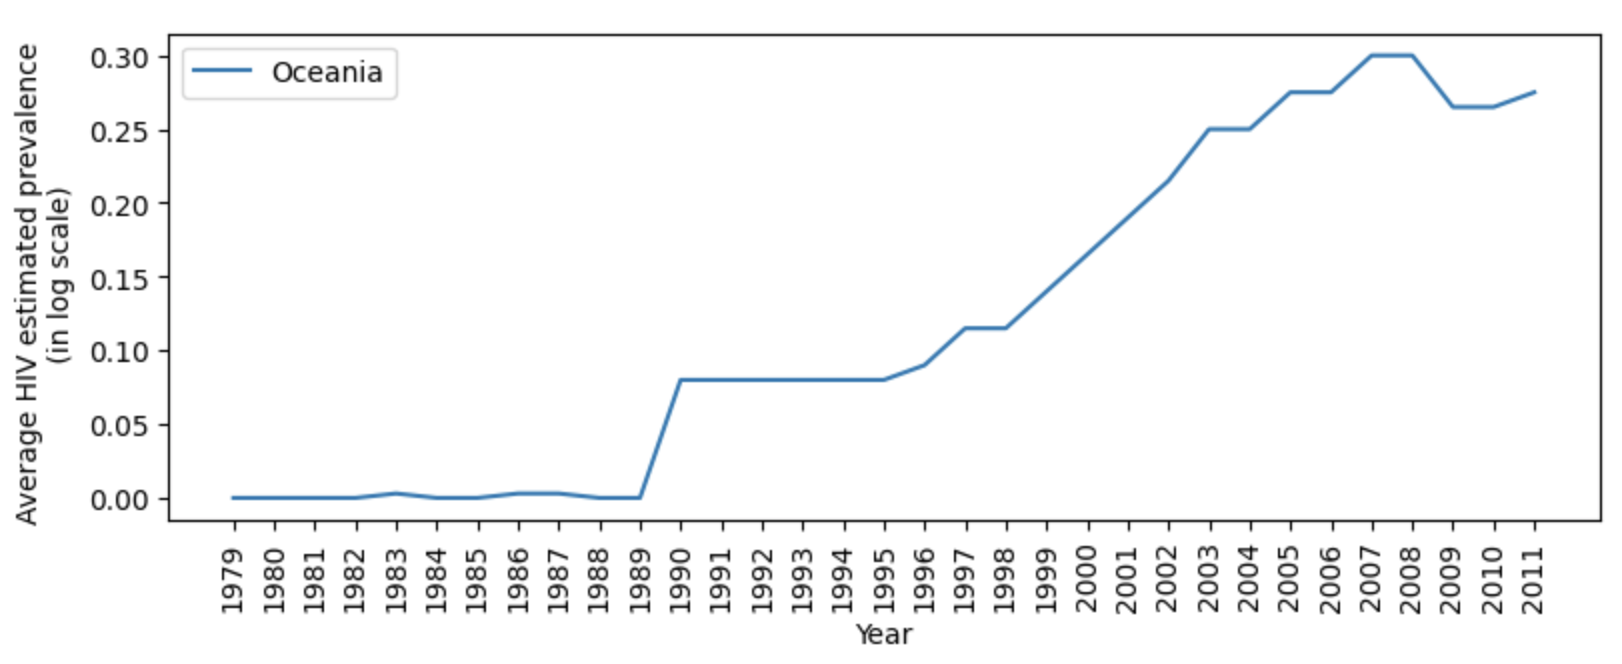
\includegraphics[width=\linewidth]{output_16.png}
		\caption{HIV data - Oceania: Changes of the average HIV estimated prevalence from 1979 to 2011 for each continent}
		\label{fig:line1}		
	\end{subfigure}
	\begin{subfigure}[b]{1\textwidth}
		\centering
		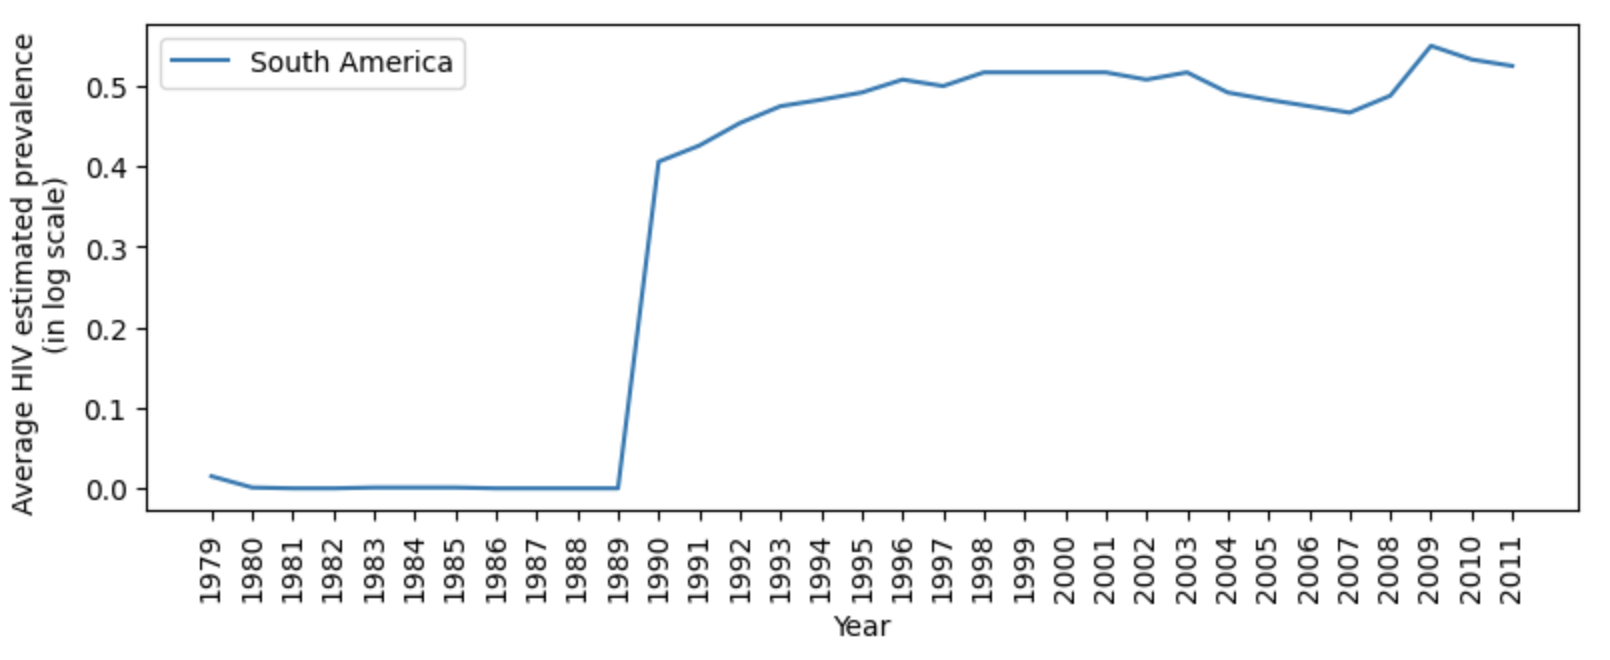
\includegraphics[width=\linewidth]{output_17.png}
		\caption{HIV data - South America: Changes of the average HIV estimated prevalence from 1979 to 2011 for each continent}
		\label{fig:line1}		
	\end{subfigure}					
\end{figure}



\pagebreak
\begin{codeblock}
\begin{minted}{python}
fig, ax = plt.subplots(1,1,constrained_layout=True)
fig.set_size_inches(8, 6)
fig.set_dpi(100)
fig.suptitle('Changes of the average HIV estimated prevalence \
\n from 1979 to 2011 for each continent')

for item in lst_year_avg:
  x_data = [x[0] for x in item[1]]
  y_data = [x[1] for x in item[1]]
  ax.set(xlabel='Year', 
        ylabel='Average HIV estimated prevalence \n (in log scale)')
  ax.set_xticklabels(x_data, rotation=90)
  ax.plot(x_data, y_data, label=item[0])
  ax.legend()
\end{minted}
\end{codeblock}

\begin{figure}[h!]
	\centering
	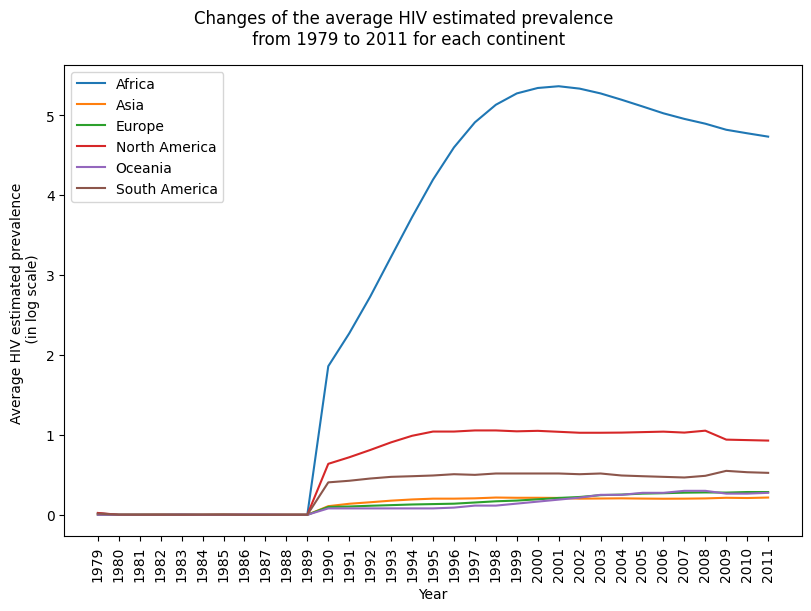
\includegraphics[width=\linewidth]{output_18.png}
	\caption{HIV data - All Continents: Changes of the average HIV estimated prevalence from 1979 to 2011 for each continent}
	\label{fig:boat1}
\end{figure}

\pagebreak
\paragraph{Task \#3}
Create two scatter plots to show the data (i.e. each country/region) in year 1990 and year 2010, respectively. The vertical axis in the scatter plot is the HIV estimated prevalence, and the horizontal axis is the corresponding year average HIV estimated prevalence in each continent, which you calculated above. Using different color to show data from different continent (1 point). If you found any interesting result from the charts, explain it.

\begin{codeblock}
\begin{minted}{python}
# preparing data
data1990 = {}
data2010 = {}
for item in lst_year_avg:
  for subitem in item:
    for subitem_year in subitem:
      if subitem_year[0] == '1990':
        data1990.update({item[0]: subitem_year[1]})
        # lst_1990data.append((item[0], subitem_year[1]))
        hiv_tbl.where('continent',item[0])
      if subitem_year[0] == '2010':
        # lst_2010data.append((item[0], subitem_year[1]))      
        data2010.update({item[0]: subitem_year[1]})
  
lst1990 = []
lst2010 = []
for row in hiv_tbl.rows:
  lst1990.append(data1990.get(row[1]))
  lst2010.append(data2010.get(row[1]))

try:
  hiv_tbl.drop('1990_continent_avg')
  hiv_tbl.drop('2010_continent_avg')
finally:
  hiv_tbl = hiv_tbl.with_column('1990_continent_avg',lst1990)
  hiv_tbl = hiv_tbl.with_column('2010_continent_avg',lst2010)

hiv_tbl.select('country','continent','1990','1990_continent_avg',
               '2010','2010_continent_avg')
\end{minted}
\end{codeblock}

\begin{figure}
	\centering
	\begin{subfigure}{1\textwidth}
		\centering
		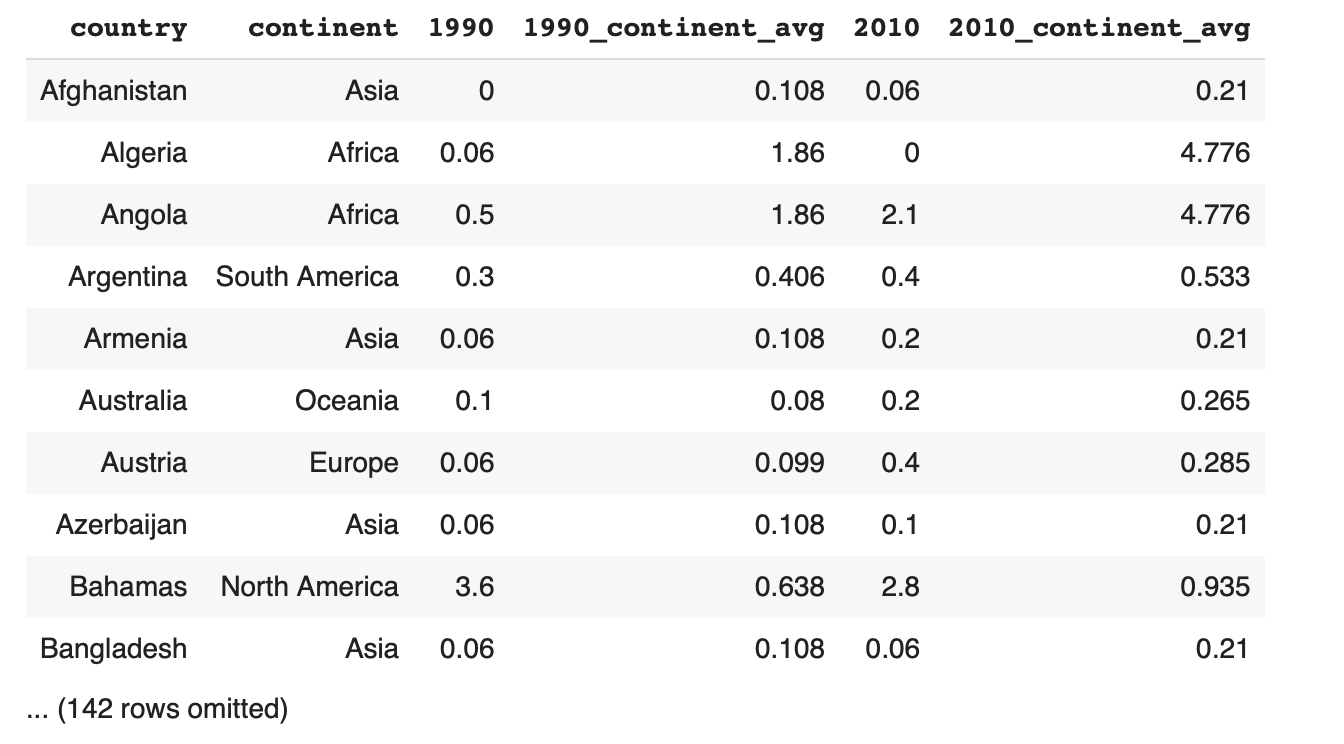
\includegraphics[width=\linewidth]{output_19.png}
		\caption{HIV data - added columns for continent average for 1990 and 2010}
		\label{fig:line1}		
	\end{subfigure}	
\end{figure}


\pagebreak
\begin{codeblock}
\begin{minted}{python}
fig, (ax1, ax2) = plt.subplots(1,2,constrained_layout=True)
fig.set_size_inches(10, 6)
fig.set_dpi(100)
fig.suptitle('HIV estimated prevalence for each country v/s \
\nAverage HIV estimated prevalence in each continent \
\n for the year 1990 and 2010')

ax1.set(xlabel='Average HIV estimated prevalence \
\n for Continents (year: 1990)', 
      ylabel='HIV estimated prevalence \
\n for Countries (year: 1990)')

ax2.set(xlabel='Average HIV estimated prevalence \
\n for Continents (year: 2010)', 
      ylabel='HIV estimated prevalence \
\n for Countries (year: 2010)')

for continent in hiv_tbl.group('continent')[0]:
  ax1.scatter(
      hiv_tbl.where('continent',continent).column('1990_continent_avg'), 
      hiv_tbl.where('continent',continent).column('1990'), 
      label=continent)
  
  ax2.scatter(
      hiv_tbl.where('continent',continent).column('2010_continent_avg'), 
      hiv_tbl.where('continent',continent).column('2010'), 
      label=continent)

ax1.legend(ncol=2)
ax2.legend(ncol=2)
\end{minted}
\end{codeblock}


\begin{figure}
	\centering
	\begin{subfigure}{1\textwidth}
		\centering
		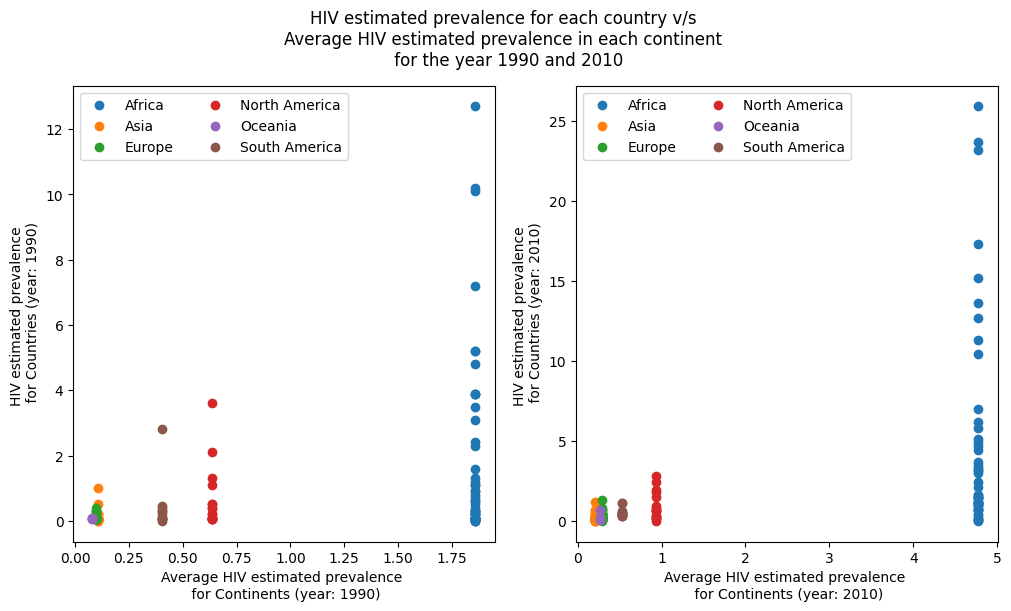
\includegraphics[width=\linewidth]{output_20.png}
		\caption{HIV estimated prevalence for each country v/s Average HIV estimated prevalence in each continent for the year 1990 and 2010}
		\label{fig:line1}		
	\end{subfigure}			
\end{figure}
	
\end{document}
